\documentclass[]{unswthesis}
\usepackage{amsmath}
\usepackage{mathtools}
\usepackage{graphicx}
\usepackage{listings}
\usepackage{color}

\definecolor{dkgreen}{rgb}{0,0.6,0}
\definecolor{gray}{rgb}{0.5,0.5,0.5}
\definecolor{mauve}{rgb}{0.58,0,0.82}

\lstset{frame=tb,
  language=Haskell,
  aboveskip=3mm,
  belowskip=3mm,
  showstringspaces=false,
  columns=flexible,
  basicstyle={\small\ttfamily},
  numbers=none,
  numberstyle=\tiny\color{gray},
  keywordstyle=\color{blue},
  commentstyle=\color{dkgreen},
  stringstyle=\color{mauve},
  breaklines=true,
  breakatwhitespace=true,
  tabsize=3
}

%%% Class options:

%%  undergrad (default)
%%  hdr

%%  11pt (default)
%%  12pt

%%  final (default)
%%  draft

%%  oneside (default for hdr)
%%  twoside (default for undergrad)


%% Thesis details
\thesistitle{Implementing neural networks in Accelerate}
\thesisschool{School of Computer Science and Engineering}
\thesisauthor{Ji Yong Jeong}
\thesisZid{z2250189}
\thesistopic{3733}
\thesisdegree{Bachelor of Engineering in Software Engineering}
\thesisdate{\today}
\thesissupervisor{A/Prof.\ Gabriele Keller}


%% My own LaTeX macros, definitions, etc
%%%% Shortcuts
\newcommand{\num}[2]{\mbox{#1\,#2}}			% num with units

%%%% Symbols
\newcommand{\yes}{\ensuremath{\surd}\xspace}		% Tick mark
\newcommand{\no}{\ensuremath{\times}\xspace}		% Cross mark
\newcommand{\by}{\ensuremath{\times}\xspace}		% XXX x XXX
\newcommand{\bAND}{\ensuremath{\wedge}\xspace}		% Bool. /\
\newcommand{\bOR}{\ensuremath{\vee}\xspace}		% Bool. \/
\newcommand{\becomes}{\ensuremath{\rightarrow}\xspace}	% -->

%%%% Custom environments

% Centered tabular with single spacing
\newenvironment{ctabular}[1]
    {\par\begin{sspacing}\begin{center}\begin{tabular}{#1}}%
    {\end{tabular}\end{center}\end{sspacing}}


%%%% Our default level for display in TOC - subsubsections
\setcounter{tocdepth}{2}



\begin{document}

%% pages in the ``frontmatter'' section have roman numeral page number
\frontmatter  
\maketitle

\chapter*{Abstract}\label{abstract}

Parallel programming, including GPU programming, is commonly used to speed up neural network computations. However, the main languages for GPU programming are CUDA and OpenCL, which are very low-level languages that are cumbersome to use. This thesis includes the implementation of a feed-forward back-propagation neural network using Accelerate. Accelerate is an Embedded Domain-Specific Language in Haskell for high performance computing and has several accessibility advantages over CUDA, while still offering competitive performance on both GPUs and CPUs using LLVM. I assess its performance, benefits and disadvantages against the traditional approaches with CUDA and other languages. Future work includes the implementation of more sophisticated networks such as convolutional neural networks on top of this foundation.

\chapter*{Acknowledgements}\label{ack}

First, I would like to express my deepest thanks to my supervisor, Gabriele Keller for her gentle encouragements, patience and guidance. I would like to thank Trevor McDonnell and Liam O'Connor for their encyclopedic knowledge and superbness. 

Also much love and thanks to my parents and sister for their long-suffering patience and support.
\chapter*{Abbreviations}\label{abbr}
\begin{description}
\item[BGD] Batch gradient descent learning algorithm
\item[CUDA] Computer Unified Device Architecture
\item[DNN] Deep neural network
\item[EDSL] Embedded domain-specific language
\item[FFBP] Feed-forward back-propagation algorithm
\item[GPU] Graphics Processing Unit
\item[OpenCL] Open Computing Language
\item[PLS] UNSW Programming Languages and Systems group
\item[ReLU] Rectified Linear Unit activation function
\item[SGD] Stochastic gradient descent learning algorithm
\end{description}

\tableofcontents
\listoffigures  % if required
%\listoftables  % if required

%% pages in the ``mainmatter'' section have arabic page numbers and chapters are numbered
\mainmatter

\chapter{Introduction}\label{ch:intro}

%% SELL THE TOPIC (1-2 pp)
Neural networks are widely used for computer vision and one of the best methods for most pattern recognition problems~\cite{Nvi14}. For instance, Deep neural networks (DNN) can already perform at human level on tasks such as handwritten character recognition (including Chinese), various automotive problems and mitosis detection.

One issue with DNN is its compute-intensiveness. Training a neural network with massive numbers of features require a lot of computations. Unfortunately, the most efficient and economical approach to testing the validity of many hypotheses is repeated trial-and-error~\cite{Ng12}.

For the above reason, neural networks are commonly engineered to make use of multicore parallelism, on both CPUs and GPUs. GPUs offer thousands of cores, and as such GPU-accelerated neural networks are generally faster than neural networks on a CPU cluster. The main languages for GPU programming are the Compute Unified Device Architecture (CUDA) from NVIDIA and the Open Computing Language (OpenCL). Both are very low-level languages based on C/C++. 

On the other hand, Accelerate is a embedded domain-specific language (EDSL) created for high-performance GPU and CPU programming inside Haskell, with higher level semantics and cleaner syntax, while still offering competitive performance. 

Thus, the motivations for this thesis is to explore the feasibility of implementing a neural network in a more on-the-fly, user-friendly approach using Accelerate. If successful, it may enable us test neural network hypotheses in a more convenient manner. 

As an initial prototype, a feed-forward back-propagation (FFBP) neural network implementation has recently been made~\cite{Eve16}, but it suffers from very poor accuracy. My project is to construct a network with competitive accuracy and performance to existing mature network implementations. 

The following section, Chapter~\ref{ch:background} outlines the background relating to this topic, from a general overview of neural networks and the mathematics behind FFBP algorithm to an overview of the Accelerate language and the previous implementation using Accelerate.

Chapter~\ref{ch:impl} introduces my implementation, discusses some issues in encoding the algorithm in Accelerate's combinator language, and identifies areas that need further development. Chapter~\ref{ch:results} discusses the testing and analysis of my network implementation, and Chapter~\ref{ch:eval} compares and contrasts my implementation with other mature neural network implementations in terms of accuracy, speed, and scalability.

Finally, Chapter~\ref{ch:conclusion} summarises the contents of this report.

\chapter{Background and Related Works}\label{ch:background}

\section{Neural network architecture}\label{sec:nn-architecture}

Broadly speaking, a neural network can be described as a certain layering of nodes, or \textit{units}, connected to each other by directed \textit{links}, where each link has a certain numeric weight that signifies the strength of connection between the connected nodes. 

Historically, the concept of `net of neurons' whose interrelationship could be expressed in propositional logic was first proposed by~\cite{McDPit43} in 1943, inspired by a ``all-or-none" behaviour of the biological nervous system. The first basic unit, also called the \textit{perceptron}, was invented by~\cite{Ros62}. A perceptron will be activated if the sum of all the input values from its input links, say $x_1,..., x_m$, multiplied by the links' corresponding weights, say $\theta_1,..., \theta_m$, is above that unit's certain threshold value, or \textit{bias} $b$, such that
\[ \text{output} = 
   \begin{cases}
   0 & \quad \text{if } \displaystyle\sum_{i=1}^{m} x_i \theta_i \leq b\\
   1 & \quad \text{otherwise }
   \end{cases}
\]

The above is equivalent to vectorizing the inputs to $\boldsymbol{x} = [x_1,...,x_m]$, weights to $\boldsymbol{\theta} = [\theta_1,...,\theta_m]$ and inverting the sign on $b$, so that,
\[ \text{output} = 
   \begin{cases}
     0	& \quad \text{if } \boldsymbol{x} \cdot \boldsymbol{\theta} + b \leq 0\\
     1	& \quad \text{otherwise }
   \end{cases}
\]

\begin{figure}
  \centerline{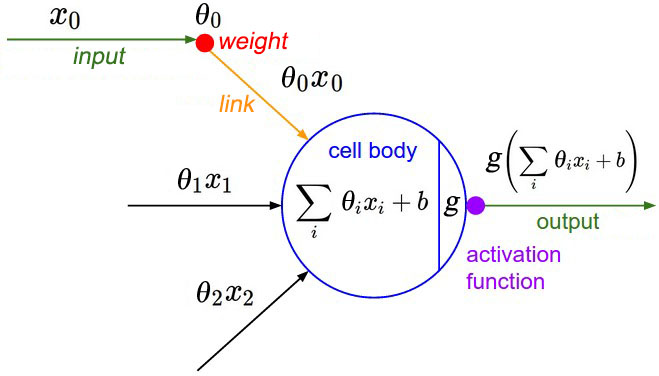
\includegraphics[width=0.7\linewidth]{neuron_model.jpg}}
  \caption{Structure of a modern unit by~\cite{Kar16}.}
  \label{fig:neuron}
\end{figure}

The perceptron eventually evolved into the modern unit, which computes the output value as a \textit{range} of values, obtained by applying an \textit{activation function} to the sum of its inputs and bias. With this modification, a small change in the inputs only resulted a small change in the output, allowing a more convenient way to gradually modify the weights and consequently, improve the learning algorithm~\cite{Nie16}.

There are various activation functions; historically, the most commonly used is the \textit{sigmoid} function, $\sigma(x) = 1/(1+e^{-x})$. Its advantages and disadvantages are outlined in \ref{se:previmplem}.~\cite{Kar16} recommends using less expensive functions with better performance, such as,
\begin{enumerate}
\item Tanh function, $tanh(x) = 2\sigma(2x)-1$.
\item Rectified Linear Unit (ReLU) function, $f(x)=max(0,x)$.
\item Leaky ReLU function, $f(x) = 1(x < 0)(\alpha x) + 1(x >= 0)(x)$
\item Maxout function, $max(w_{1}^{T}x + b_{1}, w_{2}^{T}x+b_{2})$.
\end{enumerate}

\begin{figure}
  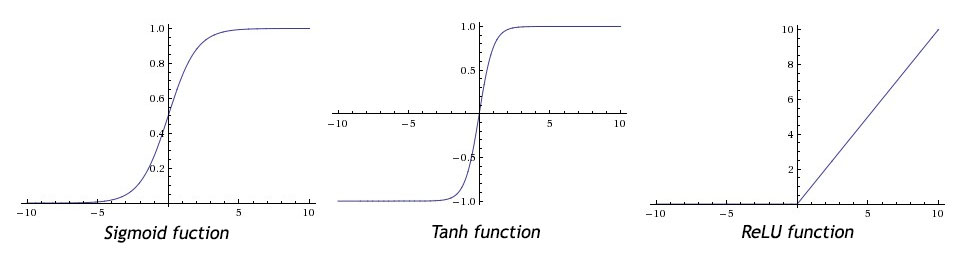
\includegraphics[width=\linewidth]{activation-functions.jpg}
  \caption{Graphs of some common activation functions~\cite{Kar16}.}
  \label{fig:activation-graphs}
\end{figure}

A unit's output can be expressed as $g(\boldsymbol{x} \cdot \boldsymbol{\theta} + b)$, where $g(x)$ is the chosen activation function.

As previously mentioned, the general architecture of a neural network can be described as distinct layers of these units, which are connected to units in its adjacent layers. The most common layer type is \textit{fully-connected}, which means that each unit in a layer is connected to every unit in the adjacent layer~\cite{Nor14}. 

The \textit{input layer} receives input values corresponding to the number of features\footnote{For instance, in a $200 \times 200$ pixel image recognition problem, there may be $40,000$ features corresponding to each individual pixel's RGB values.} in the neural network. The last, or \textit{output layer} usually corresponds to different classes in a multi-classification problem, or some real-valued target in a regression problem~\cite{Kar16}. The layers in between input and output layers are called \textit{hidden layers}; a neural network is classified as DNN if it contains more than one hidden layer. Increasing the size and numbers of hidden layers also increases the \textit{capacity} of the neural network~\cite{Kar16}; that is, the space of its representable functions. However, this may undesirably result in \textit{overfitting}\footnote{Overfitting refers to modeling the learning algorithm to excessively fit to the training samples. It thereby increases the risk of including unnecessary noise in the data, resulting in more inaccurate model.}. In the implementation (see Chapter~\ref{ch:impl}), there is a $\lambda$ or \texttt{lambda} parameter that adjusts the degree of overfitting to the training data set, which is set at the user's discretion.

\begin{figure}
  \centerline{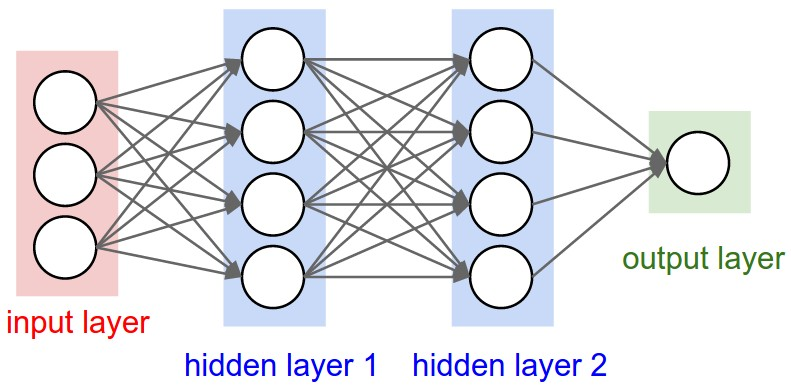
\includegraphics[width=0.7\linewidth]{neural_net2.jpeg}}
  \caption{An example of a 2-layer neural network~\cite{Kar16}.}
  \label{fig:neural-network}
\end{figure}

There are numerous neural network classifications depending on their architecture; the design relevant to this thesis is \textit{supervised}\footnote{As in ``supervised learning", a concept in machine learning where a set of training examples is paired up with a set of corresponding desired output values. A supervised neural network thus adjusts its links' weights to get the correct output values during its training phase.} FFBP neural network. Its training process and mathematical representation are briefly outlined in \ref{sec:training}.

Finally,~\cite{Nor14} summarises the attractiveness of neural networks as follows: (1) its capacity to support parallel computation; (2) its fault tolerant nature against novel inputs; (3) \textit{Graceful degradation}, which means a gradual performance drop-offs in worsening conditions; and, (4) The usage of inductive learning algorithms to train the networks.

\section{Feed-forward back-propagation learning algorithm}\label{sec:training}

This section explains the mechanics and the mathematical representation involved in training a fully-connected, supervised FFBP neural network, based on the works in~\cite{Ng12}. Given a set of features and training samples, this learning algorithm aims to find the correct weight distribution in the neural network in two stages: \textit{feed-forward propagation} and \textit{back-propagation}. 

First, the weights are randomly initialised within the permitted range of the chosen activation function. For example, this range is $[0,1]$ for a sigmoid function; for a tanh function, it is $[-1,1]$. 

Now, in a $k$-layer neural network, let the size or the number of units in layer $j$ be denoted as $|j|$. Let a particular training sample, $s$, be denoted as $(\boldsymbol{x}^{(s)},\boldsymbol{y}^{(s)})$, such that $\boldsymbol{x}^{(s)} = [x_1^{(s)},...,x_m^{(s)}]$ is the sample input and $\boldsymbol{y}^{(s)} = [y_1^{(s)},...,y_n^{(s)}]$ is the matching desired output. Let $a_{i}^{(j)}$ be the activation value of unit $i$ in layer $j$, where $1 \leq i \leq |j|$, $1 \leq j \leq k$. Let $g(x)$ be the activation function; $\Theta_{qp}^{(j)}$ be the weight of a link from unit $p$ in layer $j$ to unit $q$ in layer $j+1$; and, let $\Theta^{(j)}=[\Theta{qp}^{(j)} \text{ for } 1\leq q \leq |j+1|, 1 \leq p \leq |j|]$ be the matrix of weights controlling function mapping from layer $j$ to $j+1$.

Then we can express $a_{i}^{(j)}$ as,
\begin{equation}
a_{i}^{(j)} = g( \Theta_{i1}^{(j-1)}a_{1}^{(j-1)} + \Theta_{i2}^{(j-1)}a_{2}^{(j-1)} + ...+\Theta_{i|j-1|}^{(j-1)}a_{|j-1|}^{(j-1)} ) \label{eq:2.1}
\end{equation}
For instance, the activation of unit $i$ in the first hidden layer can be expressed as,
$$a_{i}^{(2)} = g(\Theta_{i1}^{(1)}x_{1}^{(s)} + ... + \Theta_{im}^{(1)}x_{m}^{(s)})$$
and, in the output layer as~\cite{Ng12},
$$a_{i}^{(k)} = g(\Theta_{i1}^{(k-1)}a_{1}^{(k-1)} + ...+\Theta_{i|k-1|}^{(k-1)}a_{|k-1|}^{(k-1)})$$ 
Also, unlike the approach taken above by Ng (2016),~\cite{Kar16} states that the activation function is not commonly applied to output layer, because often the result as a real-value number received by the outer layer is the information sought by the user.

\ref{eq:2.1} can be simplified using vectorised implementation. Let the activated units in layer $j$ be denoted as $a^{(j)} = [a_{1}^{(j)},...,a_{|j|}^{(j)}]$. Then inputs to this layer can be expressed as $z^{(j)} = \Theta^{(j-1)} a^{(j-1)}$ and so $a^{(j)}$ becomes,
\begin{equation}
a^{(j)} = g(z^{(j)}) \label{eq:2.2}
\end{equation}
Forward-propagation process ends when the input values are thus propagated to the output layer. 

Next, back-propagation involves re-distributing the error value between the expected output, $\boldsymbol{y}^{(s)}$, and actual output, $a^{(k)}$, back from the output layer through the hidden layers~\cite{RumHinWil86}. This concept is based on the idea that the previous layer is responsible for some fraction of the error in next layer, proportional to the links' weights. 

Let $\delta_i^{(j)}$ denote the error value in unit $i$ in layer $j$ and $\delta^{(j)} = [\delta_1^{(j)},...,\delta_{|j|}^{(j)}]$ be the vectorised error values. Then, for $1 < j < k$,
\begin{equation}
\delta^{(j)} = (\Theta^{(j)})^{T} \delta^{(j+1)} .\!* g'(z^{(j)})
\end{equation}
where $.\!*$ is an element-wise multiplication. The error in the output layer is $\delta^{(k)} = a^{(k)} - \boldsymbol{y}^{(s)}$ and that there is no error in the first layer, because as input values, they cannot contain error.

Finally, the error in link weight $\Theta_{qp}^{(j)}$ is denoted as $\Delta_{qp}^{(j)}$, such that,
$$\Delta_{qp}^{(j)}  = a_p^{(j)}\delta_q^{(j+1)}$$
This, too, can be simplified using vectorised implementation as,
\begin{equation}
\Delta^{(j)} = \delta^{(j+1)}(a^{(j)})^T \label{eq:2.3}
\end{equation}
Back-propagation ends for $s$ when the errors from the output layer is propagated to the first hidden layer.

The FFBP learning algorithm is then repeated for all the training samples. $\Delta^{(j)}$ accumulates all the errors in the training set during this process. Once the process is finished, the final values are averaged out by the size of the training set, a \textit{regularisation term} is added, and finally the weights are updated. A regularisation term is a value that is added in gradient descent algorithm in machine learning, to prohibit features that are vastly different in its range of input values from one another from distorting the results~\cite{Ng12}. This entire process is also known as a form of \textit{batch gradient descent} (BGD) learning algorithm in machine learning~\cite{Ng12} and is the method chosen to implement my Accelerate neural network (see Chapter~\ref{ch:impl}.

There are other advanced optimization methods that can improve the performance of neural networks, but these have yet to be explored at the time of this report. As with other machine learning algorithms, the performance may also be improved with either altering various parameters, such as regularisation parameter $\lambda$ and the learning rate parameter $\alpha$, altering the number of features, gaining more training examples, adding polynomial features, or any combination of these~\cite{Ng12}. However, \textit{diagnostic analysis} is often the fastest and most economically sound method to determine which set of features is effective~\cite{Ng12}. Diagnostic analysis is a form of trial-and-error testing of features sets, or \textit{hypotheses}, with a small set of training examples to assess its performance and thus its suitability.

\section{GPU-accelerated programming and neural networks}\label{se:gpu}

Neural networks implemented with GPU-accelerated programming have shown a significant performance improvement. For instance,~\cite{OhJun04} had a 20-fold performance enhancement of a multi-layered perceptron (MLP) network to detect text using an ATI RADEON 9700 PRO in 2004. More recently,~\cite{GurFor13} showed that performance gains from parallel implementation of neural networks in GPUs are scalable with the processing power of the GPU used. Their results show that performance enhancement over the pure CPU implementation increased with data set size before reaching a plateau, a limit which they contribute to the saturation of the GPU's processing cores.

~\cite{Nvi14} explains that GPU computing is particularly well-suited to neural networks due to its massively parallel architecture, consisting of tens of thousands of cores. Thus, as single GPUs can hold entire neural network, they state that neural networks benefit from an overall bandwidth increase, reduction in communication latency, and a decrease in size and power consumption compared to a CPU cluster. Furthermore, as neural network units essentially repeat the same computation only with differing input values, the algorithm complements the GPU architecture as there is minimal need for conditional instructions that could trigger thread divergences, which can dramatically reduce the GPU throughput.

The main GPU programming language is CUDA, an API model created by NVIDIA in 2007. It has a C/C++ language style and the added benefits that it bypasses the need to learn graphics shading languages or learn about computer graphics in order to program the GPU. The alternative to CUDA is Open Computing Language (OpenCL) released in 2009; also based on C/C++, it is considered to be the more complicated language of the two, but with enhanced portability. As both languages are very low-level~\cite{Mar13}, there is a need for a way to create, manipulate and test neural networks in less complicated, more user-friendly, safer, higher-level language, such as a functional language.

\section{Accelerate}\label{se:accelerate}

Accelerate is an Embedded Domain-Specific Language (EDSL) for GPU programming, released by UNSW PLS in 2011. EDSLs are restricted languages that are embedded in a more powerful language, so as to reuse the host language's infrastructure and enable powerful metaprogramming. In the case of Accelerate, Haskell is the host language and it compiles into CUDA code that runs directly on the GPU. 

\begin{figure}
  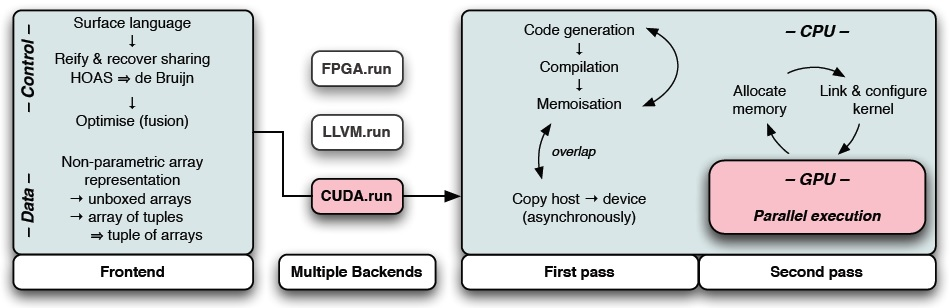
\includegraphics[width=\linewidth]{accelerate-structure.jpg}
  \caption{Structure overview of \texttt{Data.Array.Accelerate}.~\cite{ChaKelLee11}}
  \label{fig:acc-struct}
\end{figure}

Accelerate provides a framework for programming with arrays~\cite{Mar13} -- Accelerate programs take arrays as input and output one or more arrays. The type of Accelerate arrays is,
$$\texttt{data Array sh e}$$
where \texttt{sh} is the \textit{shape}, or dimensionality of the array, and \texttt{e} is the \textit{element type}, for instance \texttt{Double}, \texttt{Int} or tuples. However, \texttt{e} cannot be an array type; that is, Accelerate does not support nested arrays. This is because GPUs only have flat arrays and do not support such structures~\cite{Mar13}. 

Types of array shapes and indices are shown in Fig. \ref{fig:acc-types}~\cite{ChaKelLee11}. It shows that the simplest shape is \texttt{Z}, which is the shape of an array with no dimensions and a single element, or a scalar. A vector is represented as \texttt{Z:.Int}, which is the shape of an array with a single dimension indexed by \texttt{Int}. Likewise, the shape of a two-dimensional array, or matrix, is \texttt{Z:.Int:.Int} where the left and right \texttt{Int}s denotes the row and column indexes or numbers, respectively.

\begin{figure}
  \centerline{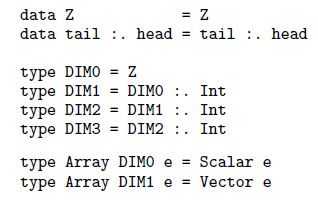
\includegraphics[width=0.5\linewidth]{accelerate-types.jpg}}
  \caption{Types of array shapes and indices~\cite{ChaKelLee11}.}
  \label{fig:acc-types}
\end{figure}

Common shapes have type synonyms, such as scalars as \texttt{DIM0}, vectors as \texttt{DIM1} and matrices as \texttt{DIM2}. Similarly, common array dimensions of zero and one also have type synonyms as \texttt{Scalar e}, \texttt{Vector e}, respectively.

Arrays can be built using \texttt{fromList}; for instance, a $2 \times 5$ matrix with elements numbered from 1 to 10 can be created with,
$$\texttt{fromList (Z:.2:.5) [1..]::Array DIM2 Int}$$

To do an actual Accelerate computation on the GPU, there are two options~\cite{Mar13}:
\begin{enumerate}
\item Create arrays within the Haskell world. Then, using \texttt{use}, inject the array \texttt{Array a} into the Accelerate world as \texttt{Acc (Array a)}. Then, use \texttt{run}.
\item Create arrays within the Accelerate world. There are various methods, such as using \texttt{generate} and \texttt{fill}. Then, use \texttt{run}.
\end{enumerate}
\texttt{run} executes the Accelerate computation and copies the final values back into Haskell after execution. In \texttt{Acc a}, \texttt{Acc} is an Accelerate data structure representing a computation in the Accelerate world, that yields a value of type \texttt{a} (more specifically, an array) \textit{once it is executed by a backend}~\cite{McD13, Mar13}. 

Now, as the first method may require the array data to be copied from computer's main memory into the GPU's memory, the second method is generally more efficient~\cite{Mar13}. All the aforementioned functions are outlined in Fig. \ref{fig:acc-functions}.
\begin{figure}
  \begin{lstlisting}
    -- build an array in Haskell world
    fromList :: (Shape sh, Elt e) => sh -> [e] -> Array sh e

	-- to execute an Accelerate computation on the GPU
    run :: Arrays a => Acc a -> a
    
    -- inject Haskell world array into Accelerate world
    use :: Arrays arrays => arrays -> Acc arrays
    
    -- create an array in Accelerate world (array filled with user-specified function)
    generate :: (Shape ix, Elt a) 
              => Exp ix -> (Exp ix -> Exp a) -> Acc (Array ix a)
    
    -- create an array in Accelerate world (array filled with same values)
    fill :: (shape sh, Elt e) => Exp sh -> Exp e -> Acc (Array sh e)
  \end{lstlisting}
  \caption{Some Accelerate functions~\cite{Mar13}.}
  \label{fig:acc-functions}
\end{figure}

Since Accelerate has its own backend compiler, it must be set before any code can be \texttt{run}. There can be a number of backends to execute Accelerate computations: (1) \texttt{Data.Array.Accelerate.Intepreter}, the slowest performing, simple Haskell interpreter; (2) \texttt{accelerate-llvm-native}, which supports parallel execution on multicore CPUs; and, (3) \texttt{accelerate-llvm-ptx}, which supports parallel execution on CUDA-capable NVIDIA GPUs. \texttt{accelerate-cuda} is deprecated in favour of (3).

Further details about the Accelerate language is continued in \ref{se:previmplem}.

\section{Previous Implementations in Accelerate} \label{se:previmplem}

A neural network in Accelerate is a fairly new concept and as such, there is only one known work in~\cite{Eve16}. In it, Everest (2016) implements a FFBP neural network with a \textit{stochastic gradient descent} (SGD) learning algorithm, based on a Python implementation~\cite{Nie16}. This section briefly covers the details of this implementation.

SGD algorithm is a modification of BGD algorithm, shown in \ref{sec:training}. Rather than adjusting the neural network parameters after going through the entire training set, SGD updates the parameters immediately after doing the FFBP algorithm for a single training example, which is picked at random~\cite{Ng12}. SGD can also be modified to select certain small batches of training sample at a time~\cite{LeC98}. 

As such, SGD is computationally less expensive than the BGD, and allows the training algorithms to scale better to much larger training sets~\cite{Ng12}. ~\cite{LeCBosDen89} also claims that SGD trains the neural network faster. The disadvantages of SGD are that it is said to be "less accurate" than BGD as it may take longer to reach the local/global minima, however, it is still the more popular choice due to less strain it puts on the system. Also, SGD is suitable to the work in~\cite{Eve16}, because it deals with processing data streaming.

There are six key Accelerate functions that were used and their names and operations are listed in Fig. \ref{fig:acc-functions2}. These functions were also used in my own implementation (see Chapter~\ref{ch:impl}). In particular, the functions \texttt{lift} and \texttt{unlift} are used to inject and extract a value into and out of \texttt{Exp}\footnote{\texttt{Exp} is another Accelerate data structure, that is similar to \texttt{Acc} (refer to \ref{se:accelerate}), but instead of an array, it represents an embedded \textit{scalar} computation~\cite{ChaKelLee11}.}, respectively, and are thus essential in interpreting the indices of arrays in Accelerate~\cite{Mar13}.

\begin{figure}
  \begin{lstlisting}
    -- apply supplied function element-wise to corresponding elements of two input arrays to produce a third array 
    zipWith :: (Shape ix, Elt a, Elt b, Elt c)
             => (Exp a -> Exp b -> Exp c)
             -> Acc (Array ix a) -> Acc (Array ix b) -> Acc (Array ix c)

	-- map function within the Accelerate world
    map :: (Shape ix, Elt a, Elt b)
         => (Exp a -> Exp b) -> Acc (Array ix a) -> Acc (Array ix b)
    
    -- replicate an array across one or more dimensions according to the first argument (a generalised array index)
    replicate :: (Slice slix, Elt e)
               => Exp slix -> Acc (Array (SliceShape slix) e)
               -> Acc (Array (FullShape slix) e)
    
    -- reduce the innermost dimension of an array
    fold :: (Shape ix, Elt a)
          => (Exp a -> Exp a -> Exp a) -> Exp a
          -> Acc (Array (ix:.Int) a) -> Acc (Array ix a)
          
    -- wraps a value in Exp
    lift :: Z:.Exp Int:.Exp Int -> Exp (Z:.Int:.Int)
    
    -- deconstruct Exp, get the structured value from within
    unlift :: Exp (Z:.Int:.Int) -> Z:.Exp Int:.Exp Int
  \end{lstlisting}
  \caption{Key Accelerate functions used in~\cite{Eve16}.}
  \label{fig:acc-functions2}
\end{figure}

In~\cite{Eve16}, two support functions were also created to assist forward- and back-propagation processes -- \texttt{mvm} and \texttt{cross} (see Fig. \ref{fig:acc-functions3}).
\begin{figure}
\begin{lstlisting}
  -- matrix vector multiplication function
  mvm :: (Elt a, IsNum a)
       => Acc (Matrix a) -> Acc (Vector a) -> Acc (Vector a)
  mvm mat vec
    = let Z:.h:._ = unlift (shape mat) :: Z:.Exp Int:.Exp Int
    in A.fold (+) 0 $ A.zipWith (*) mat (A.replicate (A.lift (Z:.h:.All)) vec)
  
  -- vector multiplication function
  cross :: Acc (Vector Float) -> Acc (Vector Float) -> Acc (Matrix Float)
  cross v h = A.zipWith (*) (A.replicate (lift (Z:.All:.size h)) v)
                               (A.replicate (lift (Z:.size v:.All)) h)
\end{lstlisting}
  \caption{Support functions for forward- and back-propagation used in~\cite{Eve16}.}
  \label{fig:acc-functions3}
\end{figure}
In \texttt{mvm}, \texttt{h} first stores the row number of the matrix input using \texttt{unlift}. The vector input, \texttt{vec} is then replicated \texttt{h} times across the first dimension using \texttt{replicate}. The resulting matrix is then element-wise multiplied with \texttt{mat} using \texttt{zipWith}. Lastly, the values of the matrix are summed and flattened back into a vector using \texttt{fold}.

The process is similar in \texttt{cross}. \texttt{cross} is a vector multiplication function that returns a matrix. First, vector \texttt{v} is replicated $|h|$ number of times in the second dimension, whereas vector \texttt{h} is replicated $|v|$ number of times in the first dimension. The resulting two matrices are then element-wise multiplied using \texttt{zipWith}. 

The actual FFBP algorithm is in the function \texttt{backprop}. In \texttt{backprop}, Accelerate code (imported as \texttt{A}) seamlessly interweaves with the Haskell part (imported as \texttt{P}), as seen in Fig. \ref{fig:acc-functions4}.
\begin{figure}
  \begin{lstlisting}
  -- back-propagation part of backprop function
  nabla_b_final = A.zipWith (*) ( costDerivative (P.last activations) y) 
                                                 (A.map sigmoid' (P.last zs) )
  nabla_w_final = cross nabla_b_final ( P.last (P.init activations) )
  
  ...
  \end{lstlisting}
  \caption{Accelerate and Haskell code are mixed in~\cite{Eve16}.}
  \label{fig:acc-functions4}
\end{figure}

At the time of this report, ~\cite{Eve16} has reported some performance issues with this implementation with the success rate of digit prediction at appropriximately 50\%. The cause is yet unknown, but may possibly be due to the nature of data streaming. This implementation also purportedly running at a slower speed than an equivalent Theano implementation. Theano is a Python library that is optimised for multi-dimensional array computations, and can be optimised to use GPU for computations.
\newcommand{\liam}[1]{$\langle$ \textit{\textbf{Liam} #1} $\rangle\ $}
\chapter{Implementation}\label{ch:impl}

\section{Using a MATLAB-based neural network as reference} \label{se:impl.matlab.nn}

MATLAB, or Matrix Laboratory, is a highly doman-specific programming language, specialised to conduct numerical calculations and analysis. It was created in the 1970s, and is an imperative procedural language with a wide array of built in linear algebra operations. It is widely used among the industry and academia, particularly in science, engineering and economics.

I have used the neural network MATLAB program in Andrew Ng's Machine Learning course in Coursera as the basis of my Accelerate program~\cite{Ng12}. There are several motivations for choosing this particular implementation. 

Firstly, the MATLAB implementation clearly shows the mathematical structure of a neural network, succinctly expressing the matrix multiplication and vectorisation operations out of which a neural network is built. It was projected that, seeing as high level matrix operations can also be easily expressed in Accelerate, this implementation would be reasonably simple to adapt, and perhaps the close-in-spirit to an Accelerate implementation.

Secondly, the MATLAB implementation also included a data set with expected answers to which I can compare my own implementations. Thus, I could be assured that my implementation in Accelerate was accurate enough to be reliable, particularly in the light of the difficulty of debugging Accelerate programs. Passing this accuracy test will indicate that my small network is reliable enough to be built upon in future machine learning developments.

Thirdly, the codebase on which I am basing my implementation is from Coursera, an online course service, specifically the Machine Learning course made by Andrew Ng of Stanford University. This course has drawn wide praise for its material and presumed to be reviewed by many in the same field. The structure of the course is reliable in terms of correctness and efficiency, and implemented already in a manner that is idiomatic for the Machine Learning community. Hence, I projected that the MATLAB implementation would be optimised for the best performance.

Lastly, in terms of familiarity, I was more conversed with MATLAB than with other neural network implementations, such as Python (see~\ref{se:previmplem}), C++~\cite{Wol17}, or Haskell's \texttt{hnn} and as such I could avoid needlessly increasing the time to start the project by choosing a language I was already comfortable using and an implementation I had already studied. While researching other implementations, I found that it took more time to understand these as I had to additionally learn the language in enough detail to understand the code being written, and the implementations differed in many details from the versions with which I was familiar.

\section{Accelerate Implementation} \label{se:impl.acc}

\subsection{Neural network structure} \label{se:impl.nn.struct}

I have implemented a two-layered, fully connected simple neural network, with one hidden layer.

My implementation can easily be modified to take more than 1 hidden layer by changing the \texttt{nnCostFunction}. For instance, each extra hidden layer should only require the addition of two matrix multiplications in the feed-forward and backpropagation components, as well as the necessary steps to update the theta layer (see~\ref{fig:nnCostFunction.hiddenlayers}).

\begin{figure}
  \begin{lstlisting}
    -- current feed-forward with 1 hidden layer
    a3 :: Acc (Matrix Float)
    a1 = xs 
    z2 = theta1 <> transpose a1 
    a2 = (fill (lift (Z :. h :. constant  1)) 1 :: Acc (Matrix Float)) 
         A.++ (A.transpose $ A.map sigmoid z2) 
    z3 = a2 <> A.transpose theta2 
    a3 = A.map sigmoid z3
    
    -- an example feed-forward with 2 hidden layers
    a4 :: Acc (Matrix Float)
    a3' = (fill (lift (Z :. h' :. constant  1)) 1 :: Acc (Matrix Float))
          A.++ (A.transpose $ A.map sigmoid z3)
    z4 = a3' <> A.transpose theta3
    a4 = A.map sigmoid z4
    
    -- an example backpropagate with 2 hidden layers
    d4 = A.zipWith (-) a4 ys
    d3 = A.zipWith (*) 
         (d4 <> theta3)
         ((fill (lift (Z :. h' :. constant  1)) 1 :: Acc (Matrix Float)) 
           A.++ (A.transpose $ A.map sigmoidGradient z3)) 
    d2 = A.zipWith (*) 
         (d3 <> theta2)
         ((fill (lift (Z :. h :. constant  1)) 1 :: Acc (Matrix Float)) 
           A.++ (A.transpose $ A.map sigmoidGradient z2)) 
  \end{lstlisting}
  \caption{Changing the number of hidden layers in \texttt{nnCostFunction}}
  \label{fig:nnCostFunction.hiddenlayers}
\end{figure}

\subsection{Program structure} \label{se:impl.program.struct}

In terms of program structure, I closely followed the control flow of the MATLAB version. It can be partitioned into three main subroutines: (1) initialisation; (2) the neural network cost function; and, (3) function minimisation via the conjugate gradient method. The implementation code is available at~\cite{McDJeo}.

\subsubsection{Initialisation} \label{se:impl.init}

Initialisation is a straightforward process. We initialise (1) the regularisation parameter \texttt{lambda}; (2) initial weight vectors, in this instance \texttt{theta1} and \texttt{theta2}; (3) size of the input, hidden, output layers; and, (4) the input training data set \texttt{xs} and the output vector \texttt{ys} to conduct the supervised learning. 

The number of input units correspond to the number of attributes in each sample of \texttt{xs}, whereas the output units correspond to the number of classifications that these samples could be divided into, or, the range of the values of \texttt{ys}. Setting the number of neurons in the hidden layer is mostly done by a mixture of guesswork and trial-and-error. In \ref{se:res.testdata}, 25 and 300 neurons comprise the hidden layer for two different data sets of handwritten numbers. These sizes were taken from other implementations with the same data sets, who had found these the most effective numbers by testing.

The matrix \texttt{xs} represents $m$ training set data. After it has been loaded, each row of \texttt{xs} should represent a single training example, $x_1, x_2, ..., x_m$ where the length of vector $x_i$ is the size of the input layer. A column vector of $1$s is added to the leftmost of the array to represent the bias neuron, as shown below.
\[
 \texttt{xs} =
    \begin{bmatrix}
      1 \\
      1 \\
      ... \\ 
      1
    \end{bmatrix}
    \begin{bmatrix}
       x_1 \\
       x_2 \\
       ... \\
       x_m
    \end{bmatrix}
\]

This is implemented in Accelerate using a combination of \texttt{fill} and concatenation \texttt{A.++}. Accelerate's operations are not the same as Haskell Prelude's, even if some operation names coincide. Thus they are distinguished by a qualified import: \texttt{A}, \texttt{P} for Accelerate and Prelude correspondingly, for instance \texttt{A.++} and \texttt{P.++}. Other key array manipulation functions used throughout the program include \texttt{A.take, A.drop, A.map} and \texttt{A.zipWith}.

In contrast to the clarity of the underlying structure offered by Accelerate's syntax, MATLAB functions automatically apply multiplications of a scalar term to a matrix, by applying the operation of the scalar to each element of the matrix. Thus, if \texttt{a} is a scalar and \texttt{xs} is a matrix, it is possible to simply do \texttt{a} $\times$ \texttt{xs}. In Accelerate, this would be \texttt{A.map (*a) xs}. As a result, MATLAB code is deceptively compact --- it may not reveal the actual structure of the underlying operation just from a surface examination of the program syntax. 

Other notable MATLAB difference is the starting index of matrices and arrays being $1$, not $0$.

The effectiveness of the random initialisation of weight vectors will influence the accuracy of the neural network. Initial values should be in the range $[-\epsilon_{init}, \epsilon_{init}]$~\cite{Ng12}. One popular choice of $\epsilon_{init}$ is,
\[ \epsilon_{init} = \sqrt{\frac{6}{L_{in} + L_{out}}} \]
where $L_{in}$ is number of units in the preceding layer, and $L_{out}$ is the number of units in the subsequent layer of the weight vector-in-question. 

The optimal regularisation parameter \texttt{lambda} is also discovered by trial-and-error. It is set by the user to determine the level of fitting of the neural network to the training set is considered `overfitting'. Whether higher or lower overfitting to the training set is better or worse for making predictions on new samples depends entirely on the nature of the data. 

\subsubsection{Neural network cost function, \texttt{nnCostFunction}} \label{se:impl.nnCostFunction}

This function applies both the feed-forward and back-progapation to sample data inputs and updates the weight vectors and error costs accordingly. 

As described in \ref{sec:training} we apply the BGD method by grouping all the sample data into one large batch, passing them in all at once, for higher accuracy. 

As the \texttt{nnCostFunction} is used in conjunction with the \texttt{fmincg} function (\ref{se:impl.fmincg}), it was necessary to flatten all the weight vectors into a single dimension before passing them into, and returning them from the \texttt{nnCostFunction}. The flattened vector is sliced and reshaped to restore the vectors to their original shapes inside \texttt{nnCostFunction}, implemented via the Accelerate \texttt{reshape} function as shown in~\ref{fig:reshape}.

\begin{figure}
	\begin{lstlisting}
	-- type of reshape
    reshape :: (Shape sh, Shape sh', Elt e) =>
                Exp sh -> Acc (Array sh' e) -> Acc (Array sh e)

    -- unroll theta1, theta2
    theta1 = reshape (index2 hiddenl (inputl +1)) $ A.take (hiddenl*(inputl+1)) thetas
    theta2 = reshape (index2 outputl (hiddenl+1)) $ A.drop (hiddenl*(inputl+1)) thetas
	\end{lstlisting}
  	\caption{Reshaping vectors into matrices in Accelerate.}
	\label{fig:reshape}
\end{figure}

Using \texttt{reshape} can be initially cumbersome, because it must be supplied with an \texttt{Exp} of the output shape. This can be supplied in various ways, and may require its type to be explicitly specified. For example, in the case where one \texttt{lift}s a \texttt{(Z:.m:.n)} expression to supply \texttt{fill} with an \texttt{Exp (Z:.Int:.Int)}, a type signature is required:
$$\texttt{fill (lift (Z:.m:.n)) 1 :: Acc (Matrix Float)}$$
Thus, I found operations involving shape parameters quite tricky at times due to the necessity of explicit typing.

Matrix multiplications was initially implemented using \texttt{mmult}, but to improve performance on the CPU LLVM backend, the foreign function interface of Accelerate ~\cite{Eve16} was used to call the matrix multiplication function from the \texttt{hmatrix} package, which has a better performance. 

\subsubsection{Function minimisation via conjugate gradient method, \texttt{fmincg}} \label{se:impl.fmincg}
Generally, function minimisation by conjugate gradients is a quadratically convergent gradient method used to locate a local minimum when the function has several variables, or, is \textit{multivariate}~\cite{FleRee}. This function repeats \texttt{nnCostFunction}, a multivariate function, for certain number of iterations, and progressively tries to minimise the error in the weight matrices.

In MATLAB, function minimisation by conjugate gradient is a function called \texttt{fminunc}, which states that given a starting point \texttt{x0} (can be a scalar, vector or a matrix), \texttt{x} is the local minimum of unconstrained function \texttt{func}~\cite{Mat17}:
$$\texttt{x = fminunc(func, x0)}$$
\texttt{fmincg} function is a modified version of \texttt{fminunc} and has the following MATLAB equation:
$$\texttt{function [X, fX, i] = fmincg(f, X, options, P1, P2, P3, P4, P5)}$$
According to the author, it is more efficient than \texttt{fminunc} in that it uses `Polack-Ribiere' conjugate gradients, quadratic and cubic polynomial approximations and the `Wolfe-Powell stopping criteria' to more efficiently calculate slope and stepping sizes~\cite{Reb13}. The mathematics behind this method is beyond the scope of my understanding.

The \texttt{fmincg} function terminates when it either finds the local minimum, or if the progress is so insignificant that it is not worth any further exploration. It must be given a cost function \texttt{f}, initial weight vector \texttt{X} and maximum iteration number in \texttt{options}. Other parameters are not supplied. 

The function returns the solution vector as \texttt{X} and a cost vector as \texttt{fX}. \texttt{fX} starts off as an empty vector, and \texttt{fmincg} pushes the cost/error of the newly recalibrated weights in each iteration to the back of \texttt{fX}. The end result is that the caller can see the progress made throughout the iterations by checking \texttt{fX}. Other variables are discarded.

The Haskell/Accelerate type signature of \texttt{fmincg} can be seen in~\ref{fig:fmincg}. The vector argument is a concatenation of flattened weight matrices and is fed into the function argument. This is to enable \texttt{fmincg} to execute the function independently from the structure of the underlying neural network, i.e. the number of hidden layers. It is a artifact of MATLAB methodology that needs better implementation in Accelerate (see Chapter~\ref{ch:eval}).

\begin{figure}
	\begin{lstlisting}
	fmincg :: (Acc (Vector Float) -> Acc (Scalar Float, Vector Float))
           -> Acc (Vector Float)
           -> (Acc (Vector Float), Acc (Vector Float))
	\end{lstlisting}
  	\caption{Function minimise conjugate gradient function.}
	\label{fig:fmincg}
\end{figure}

I faced a couple of challenging factors in implementing this function. First, the MATLAB version had approximately 17 parameters, most of which are overwritten and interact in complex, intricate ways. Without a knowledge of the underlying mathematics, I could not fully comprehend the overall structure of this 175-line procedure. The ambiguity and similarity of parameter names, such as \texttt{d1,d2,...,v3}, did nothing to ease the problem. 

Secondly, it is difficult to follow the flow of control in \texttt{fmincg}. In order to reduce the chance of errors arising, I chose to initially follow the procedure very closely, hoping to optimise incrementally later. Certain expressions were substituted where operations had not yet been implemented in Accelerate (see~\ref{se:impl.limits}). Additionally, I could not model the extremely complex flow control perfectly, and the known issues and bugs are mentioned in~\ref{se:impl.limits}.

Thirdly, MATLAB \texttt{fmincg} was composed of three \texttt{while} loops within each other and three \texttt{if-else} statements, one of the latter which resulted in a flow divergence. The last factor in particular may have greatly reduced this implementation's suitability for GPU execution, as such parallelism with flow divergence may can cause drastic problems in GPU performance, which favours non-divergent \emph{flat-data parallelism}, where sequential operations can be applied in parallel over bulk data.

On the positive side, the flow divergence is only triggered upon a failure to find a local minimum; which, according to~\cite{Reb13} occurs when the function supplied to \texttt{fmincg} is inaccurate or unsuitable. For this particular implementation, I have taken the assumption that the function supplied, \texttt{nnCostFunction} is accurate and that there is always a local minimum that \texttt{fmincg} will find. In my limited tests (see Chapter~\ref{ch:results}), all results support this assumption. More broadly, the correctness of the function can be checked for prior to being supplied to \texttt{fmincg}.

To make my implementation more manageable, I divided the MATLAB code into their \texttt{while} loops. These were implemented using Accelerate's \texttt{awhile} flow control combinator. 

This combinator \texttt{awhile} requires variables that change during the loop and/or are returned when function ends, to be wrapped into a single \texttt{Acc} tuple to be used for the loop process. The functions \texttt{lift} and \texttt{unlift} are necessary to pack and unpack the variables respectively in each loop, for condition checks and for loop execution. An interesting fact I learnt was that Haskell's type inference quickly meets its match with Accelerate --- it cannot infer the types of some variables unless they are unambiguously used after an \texttt{unlift} call. It is thus sometimes necessary to specify types of certain terms to assist Haskell with type inference as seen in~\ref{fig:unlift}.

\begin{figure}
	\begin{lstlisting}
    d1, f1, limit :: Acc (Scalar Float)
    m :: Acc (Scalar Int)
    (theta, df2, d1, d2, d3, f1, f2, f3, z1, z2, z3, m, limit) = unlift $ awhile cond body initial
	\end{lstlisting}
  	\caption{Assisting Accelerate by specifying types of unused variables in \texttt{unlift}.}
	\label{fig:unlift}
\end{figure}

\section{Known bugs} \label{se:impl.limits}

There are several issues with my Accelerate implementation. One, it does not have the robust failure handling, allowing it withstand incorrect inputs analogously to the MATLAB programs. For instance, I have already mentioned in \ref{se:impl.fmincg} that the function supplied to \texttt{fmincg} must have a clear minimum. 

Also, there are cases in \texttt{fmincg} where some variables need to checked for \texttt{isinf}, \texttt{isreal} or \texttt{isnan}, that is, be checked for an infinity, a real number, or 'not-a-number' floating-point properities, respectively. As these functions are not yet available in Accelerate, I substituted them for expressions which I believe will cover those particular situations. For instance, \texttt{isreal} check may arise when a determinate may be less than zero; \texttt{isnan} may arise when a divisor is zero. I was not able to devise a check for \texttt{isinf}, however, so the implementation may not cover all the range of inputs and remain fault-free.

Secondly, MATLAB's \texttt{double} is by default a double-precision data type, and requires 64 bits~\cite{Mat17}. Yet, after testing it on the sample data, importing the values in Accelerate as \texttt{Double}s produces a result further away from the MATLAB result than when I pass them to Accelerate as \texttt{Float}s. Not only that, the accuracy of the Accelerate neural network predictions after training decreased with the same training set when the data was passed as a \texttt{Double}. 

The source of the inaccuracy may be due to \texttt{fmincg}. There is one line that seems to account for overflow, by subtracting \texttt{realmin} from a dividend as seen in~\ref{fig:realmin}. The value \texttt{realmin} for a \texttt{float} is defined as $1.1755e^{38}$ and for a \texttt{double} is $2.2251e^{308}$ in MATLAB. These different by orders of magnitude ($1xe^{270}$) and could vastly affect the result. In my implementation, I have currently taken out \texttt{realmin} from the equation, which increases the risk of division by zero but does not seem to be problematic in practice.

\begin{figure}
	\centerline{
\includegraphics[width=\linewidth]{realmin.png}}
	\caption{MATLAB's \texttt{double} is actually a \texttt{float}? What it means for \texttt{realmin}.}
	\label{fig:realmin}
\end{figure}

Lastly, some of the optimisations in \texttt{fmincg} has been ignored, namely: (1) the innermost and middle loop iterations, thus the loop counter \texttt{M} is set to 1; and, (2) the handling of a failure case. The reason for (2) has already been discussed in \ref{se:impl.fmincg}. For (1), testing has shown that the iterations other than exactly once for the sections in question produces erroneous results, and the reasons for this is unfortunately still unknown at the time of writing. In addition, although setting \texttt{M=1} seems to closely align my program's results to MATLAB's results in the first training set, my neural network was unable to yield as high accuracy rate as in ~\cite{LeC98} for the second training set, deviating by almost 10 per cent (see Chapter~\ref{ch:results}, ~\ref{ch:eval}).

\section{Other works}
I have also implemented a logistic regression cost function, which is akin to a neural network without any hidden layers. This can be accessed at ~\cite{McDJeo}. This function produces analogous results to the equivalent MATLAB implementation.
 %% thesis B results
\chapter{Testing and Results}\label{ch:results}

\section{Test Data}\label{se:res.testdata}
There are two data sets that I have tested the implementation with: (1) handwritten digits data set from~\cite{Ng12}; and, (2) handwritten digits data set from~\cite{LeCCorBur}.

(1) is a $5000$ training examples of $20 \times 20$ pixel greyscale images of digits, each pixel represented by a floating point number that indicates the greyscale intensity at that location. The input layer will thus have 400 neurons. Hidden layer has 25 neurons and the output layer has 10 neurons. The output neuron with the highest activation value will be the digit that the sample will be classifed as. For instance, if the neuron 4 of the output vector, \texttt{ys[3]} had the highest value, then the sample will be classified as digit 4.

\begin{figure}
	\centerline{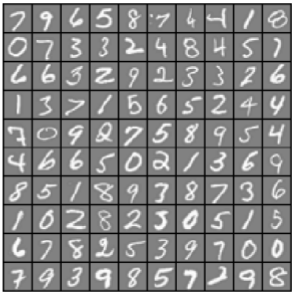
\includegraphics{ng-dataset.png}}
	\caption{An example representation of the handwritten digits data set from~\cite{Ng12}.}
	\label{fig:ng.data}
\end{figure}

This data set was mostly used during the development to assess the accuracy of the implementation, as I could easily check the values that I get from my program with the values in the MATLAB program. In ~\ref{se:res.performance} I evaluated the comparative performance of Accelerate and MATLAB, up to 2 cores.

(2) is Le Cunn's MNIST handwritten digits database. This consists of a training set of $60000$ examples and a test set of $10000$ examples. Each example is a $28 \times 28$ pixel greyscale images written by $250$ writers. This input layer has 784 neurons and a hidden layer of 300 neurons. This data was used to test the performance of completed Accelerate implementation up to 8 cores.

\section{Testing environment}\label{se:res.testsys}
There are two testing environments. Both environments ran on \texttt{llvm} backends as the testing data was too small for the GPU backend. 

First is the development testing configuration. It is backed by a 2-core Intel i5-5200U CPU (64-bit, 2.2GHz, 12GB RAM, hyperthreading enabled) running GNU/Linux (Ubuntu 16.04 LTS). 

Second is a multi-core testing configuration. It is a 4-core "Ivy Bridge" Intel i7-3720QM (64-bit, 2.6GHz, 8GB SDRAM, hyperthreading enabled) running MacOS.

\section{Performance results}\label{se:res.performance}

Table \ref{tb:acc.vs.matlab} shows that the accuracy of the Accelerate implementation is similar to MATLAB's, however, the time taken to calculate the weights grows much faster depending on the sample size. This may be due to some bugs (see Chapter~\ref{ch:eval}).

\begin{table}
\centering
\resizebox{\textwidth}{!}{
	\begin{tabular}[width=\linewidth]{| r | p{3cm} | p{3cm} | p{3cm} | p{3cm} |}
    \hline
    Input size & Accelerate (LLVM-CPU)(s) & Accelerate accuracy (\%) & MATLAB (s) & MATLAB accuracy (\%) \\ \hline
     100 & 0.4912 	& 75.22 	& 0.2037 	& 75.00  \\ \hline
     250 & 0.9312	& 83.42 	& 0.3592 	& 83.84  \\ \hline
     500 & 1.545 	& 88.86 	& 0.5028 	& 88.66  \\ \hline
     750 & 2.106 	& 89.94 	& 0.7283 	& 89.94  \\ \hline
    1000 & 2.821 	& 91.40  	& 0.8276 	& 90.90  \\ \hline
    1500 & 4.052 	& 92.64 	& 1.2782 	& 92.40  \\ \hline
    2000 & 5.915 	& 93.44 	& 1.3827 	& 93.62  \\ \hline
    3000 & 8.273 	& 94.10 	& 1.9658 	& 94.50  \\ \hline
    4000 & 13.1 	& 94.74 	& 2.4011 	& 94.96  \\ \hline
    5000 & 17.95 	& 95.54 	& 2.6811 	& 95.08  \\ 
    \hline
	\end{tabular}}
	\caption{Benchmarking compared to MATLAB results.}
	\label{tb:acc.vs.matlab}
\end{table}

-- INSERT GRAPH

Table \ref{tb:acc.vs.cores} shows a tapering improvement of performance with addition of more cores. It levels off rapidly, however, perhaps indicating that there may be too much overhead to keep the cores synchronized to gain much benefit with this implementation.

\begin{table}
\centering
\resizebox{\textwidth}{!}{
	\begin{tabular}[width=\linewidth]{| c | c | c |}
    \hline
    Number of cores & Accelerate (LLVM-CPU)(s) & Accelerate accuracy (\%) \\ \hline
     1 & 239.695	& 83.97 	\\ \hline
     2 & 184.37  	& 84.46 	\\ \hline
     3 & 151.967 	& 84.46 	\\ \hline
     4 & 135.719	& 84.46 	\\ \hline
     5 & 133.421	& 84.46  	\\ \hline
     6 & 130.372 	& 84.46 	\\ \hline
     7 & 124.314 	& 84.46 	\\ \hline
     8 & 122.310 	& 84.46 	\\ 
    \hline
	\end{tabular}}
	\caption{Benchmarking under different number of cores.}
	\label{tb:acc.vs.cores}
\end{table}

 %% raw of results
\chapter{Evaluation}\label{ch:eval}

The intent of this thesis was to create a neural network in Accelerate that is (1) sufficiently well-performing; (2) with good usability; and, (3) analyse the benefits and disadvantages of such implementation. I will go through each one in the sections below.

\section{Performance evaluation} \label{se:eval.performance}

In terms of performance, namely correctness, scalability and relative speed, my implementation did not perform well as expected (see Chapter~\ref{ch:results}).

Although accuracy was on-par with MATLAB on training set (1), it had lower accuracy than other implementations, including MATLAB, on the second training set. According to~\cite{LeC98}, a two-layer fully connected neural network 300 hidden units for MNIST dataset should produce an error of approximately 4.7\%. Albeit the fact that LeCun (1998) uses a carefully tuned, SGD algorithm method named \textit{Stochastic Diagonal Levenberg-Marquardt}\footnote{This is a complex method, but amongst other techniques, LeCun (1998) calculates an individual learning rate for each weight before parsing the training set --- which is applied to the network around 20 times --- in a randomised order of \textit{patterns}, or the sorting of training samples in a properly randomised sequence.} to train his neural network, one should expect my Accelerate implementation to mirror the accuracy of MATLAB's performance as it did for training set (1). However,\ref{tb:acc.vs.cores} indicates that it is approximately 7.2\% less accurate than that of MATLAB. This seems to signify that the unresolved bugs and issues as previously mentioned in \ref{se:impl.limits} is a significant dampener on the accuracy of my implementation.

Also worth noting is that the MATLAB implementation has a higher error rate of 8.3\% compared to LeCun's SGD neural network at 4.7\%. This seems to imply that BGD with conjugate gradient method may not be as effective as SGD (or perhaps, for this particular data set). 

Interestingly, my program with an error rate of 15.5\% is closer the error rate reported by a native Haskell neural network implementation called \texttt{neural}~\cite{Bru16}. Upon testing with MNIST training set, \texttt{neural} produced an error rate of approximately 17\% after 50 iterations, taking 983.9 seconds with 8 cores. This program reports it can ultimately reach an accuracy of 90.05\% after 450 iterations. 

%Sadly, both of our accuracy rate is worse than the performance of LeCun's classic linear classifier\footnote{A linear classifier architecture is similar to a neural network without a hidden layer.} at 12\%.

In terms of scalability, my implementation linearly increases the time taken compared to size of input with constant number of cores similar to MATLAB, and reaches a plateau rapidly upon adding more (see ~\ref{fig:traininggraphs}). We believe this may be due to the rolling and unrolling of weight vectors during \texttt{fmincg} operation as mentioned in \ref{se:impl.fmincg}. The amount of work involved in copying the large matrices probably adds a significant overhead, reducing the benefit of having multicores.

Such redundant work is also likely a factor in negatively affecting the speed, particularly for smaller data sets. For instance, the MATLAB program seems to perform much faster with the smaller training set (1) (see ~\ref{fig:traininggraphs}). With MNIST training set, however, my Accelerate program does perform more competitively --- but, further testing is required. 

I was unable to find \textit{speed} performance results for MNIST training set on neural networks with same architecture in other languages in order to do a relative speed performance apart from MATLAB\footnote{The closest one I could find was a C++ neural network\cite{Wol17}, but with only 30 hidden layers. This reduces the first weight vector from $235500$ to $23550$ and the second weight vector from $3010$ to $310$. This implementation also uses the faster SGD method in the manner of~\cite{LeC98} and also did not disclaim his testing environment. Training time taken is said to be 82 seconds, but there were too many unknown factors in this data to draw comparisons.}.

Yet, on a positive note, my Accelerate neural network finishes training at 122.3 seconds with 8 cores. This is despite the fact that this implementation is more or less a direct translation of the MATLAB code with minimal Accelerate optimisation. With further Accelerate naturalisation (and bug fixes), it may be possible to achieve a very reasonable speed performance!

\section{Usability and Accelerate} \label{se:eval.usability}

It is fairly reasonable to say that the ease and convenience of a programming language can affect a programmer's work. One of the main reasons in starting this thesis was to gauge the ease of creating a neural network using Accelerate.

Firstly, Accelerate has a convenient syntax that Haskell-users will find easy to use. Although MATLAB may seem more convenient than Accelerate at times, especially in operations that requires array or matrix manipulations, MATLAB is also ambiguous and loose in its language, and meanings can get lost without more effort being invested by the reader (see ~\ref{se:impl.matlab.nn}). In contrast, Accelerate is explicit and unambiguous in its syntax, with clear dynamic semantics and a static type system to catch errors. It also has a growing collection of high performance libraries for array computations that are easy-to-use.

Secondly, Accelerate is compact and succinct, but perhaps not as abbreviated as in MATLAB to become obscure to its users. Neither is Accelerate as verbose as C++, which can become cumbersome to read and write as seen in ~\ref{fig:eval.syntax.predict}.

\begin{figure}
  \begin{lstlisting}
	-- in MATLAB
	function p = predict(Theta1, Theta2, X)
	m = size(X, 1);
	h1 = sigmoid([ones(m,1) X] * Theta1');
	h2 = sigmoid([ones(m,1) h1] * Theta2');
	[~,p] = max(h2, [], 2);
	end
	  	
	-- in Accelerate  	
  	predict :: Acc (Matrix Float) -> Acc (Matrix Float) -> Acc (Matrix Float) -> Acc (Vector Int)
    predict theta1 theta2 xs = 
    let
        Z :. m :. n = unlift (shape h1) :: Z :. Exp Int :. Exp Int
        h1 = A.map sigmoid 
           $ xs <> A.transpose theta1                
        h2 = A.map sigmoid 
           $ ((fill (lift (Z:.m:.(constant 1))) 1 :: Acc (Matrix Float)) A.++ h1)
             <>
             (A.transpose theta2)

        getYs :: Acc (Vector Int)
        getYs
          = A.map ((+1) . A.indexHead . A.fst)
          $ A.fold1 (\x y -> A.snd x A.> A.snd y ? (x , y))
          $ A.indexed h2
    in
    getYs
  	
  	-- in C++
	uint8 ForwardPass (const float* pixels, uint8 correctLabel) {
        for (size_t neuronIndex = 0; neuronIndex < HIDDEN_NEURONS; ++neuronIndex) {
            float Z = m_hiddenLayerBiases[neuronIndex];
            for (size_t inputIndex = 0; inputIndex < INPUTS; ++inputIndex)
                Z += pixels[inputIndex] * m_hiddenLayerWeights[HiddenLayerWeightIndex(inputIndex, neuronIndex)];
            m_hiddenLayerOutputs[neuronIndex] = 1.0f / (1.0f + std::exp(-Z));
        }
        
        ... 
        return maxLabel;
    }
  \end{lstlisting}
  \caption{Comparing \texttt{predict} in MATLAB~\cite{Ng12}, Accelerate and C++~\cite{Wol17}.}
  \label{fig:eval.syntax.predict}
\end{figure}

There are, however, several elements that can intimidate new users to Accelerate. For example, I found it was quite difficult to debug my program, as Accelerate computations are not observable until they are returned to Haskell world. 

Secondly, as previously mentioned in ~\ref{se:impl.fmincg}, Haskell's type inference could not automatically infer the types of some Accelerate variables, particularly in \texttt{unlift} operations. 

Other minor inconveniences include determining which situation called for \texttt{Exp} and \texttt{Acc} and why or when one should switch between those two data structures, the fact that it was not possible to extract values from \texttt{Exp}, and lastly, the initial set up was quite intimidating.

\section{Advantages of an Accelerate implementation} \label{se:eval.advantages}

There are several advantages to using Accelerate. First, it results in much simpler source programs as programs are written in Haskell syntax; Accelerate code is very similar to an ordinary Haskell code and there are minimal syntactic difference~\cite{Mar13}.

Second, as Accelerate is embedded in Haskell, it can benefit from inheriting Haskell's functional language characteristics. For instance, Haskell as a pure language is advantageous for parallel computations as it will prohibit side effects that can disrupt other threads.

Another Haskell characteristic is having a more powerful type system, which could enforce a stronger checking for certain properties --- thereby catching more errors --- at compile time. In comparison, languages like MATLAB are dynamically typed, meaning that the types may change during runtime. Futhermore, as a weakly typed programming language, its types can be implicitly converted whenever a mismatch occurs, making its program unpredictable and unreliable.

Thirdly, Accelerate uses a number of optimisation techniques to mitigate the overheads, such as array fusion and sharing recovery\cite{ChaKelLee11}. For instance, my implementation was very inefficient in the sense that it would have generated multiple copies of same variables due to many \texttt{while} loops in a non-optimising compiler. Accelerate will optimise the code to reduce the number of parameters to the bare minimum required during the production of the ASTs in compile time. It will also 'fuse' sequences of \textit{producer/producer} operations and fuse \textit{producer/consumer} operations to eliminate intermediate arrays --- overall, resulting in a much cleaner, efficient program~\cite{McDChaGro}.

Finally, Accelerate is a dynamic code generator and as such it can, (1) optimise a program at the time of code generation simultaneously by obtaining information about the hardware capabilities; (2) customise the generated program to the input data at the time of code generation; and (3) allow host programs to ``generate embedded programs on-the-fly"~\cite{ChaKelLee11}.

On the other hand, the disadvantage of using Accelerate is the extra overheads, which may originate at runtime (such as runtime code generation) and/or at execution time (such as kernel loading and data transfer)~\cite{ChaKelLee11}. Some of the overheads however, such as dynamic kernel compilation overheads, may not be so problematic in heavily data- and compute-intensive programs, because the proportion to the total time taken by the program may become insignificant~\cite{ChaKelLee11}; and, neural networks certainly fit in such a category of programs. 

Indeed, even with the small data sets in this implementation, the results in Chapter \ref{ch:results} seem to support this: for the small training set (1) the overhead outweighed the parallelism advantages, making the Accelerate implementation perform more poorly compared to MATLAB; however, Accelerate performed better than MATLAB for the larger training set (2).

\section{Incomplete works} \label{se:eval.incomplete}

As stated in ~\ref{se:impl.limits}, there are a number of issues that requires further work in my current implementation. First is resolving the unexpected behaviour in the inner and middle loops when \texttt{M} variable is not set at 1. Secondly, the rolling and unrolling of weight matrices should be optimised or eliminated, in order to reduce overhead. 

I would also test the accuracy of the predictions by trying a different activation functions. I have used the sigmoid function in this implementation, initially in order to confirm that my development is in alignment with MATLAB's and also because it is mathematically convenient, because its gradient, $\sigma'(x)$, is easy to calculate:
$$\sigma'(x) = \sigma(x) \cdot (1 - \sigma(x))$$
However, sigmoid function is not widely used these days, due to these two disadvantages~\cite{Kar16}:
\begin{enumerate}
\item When the unit's activation \textit{saturates} at either tail of 0 or 1, the gradient of the sigmoid function nears zero (refer to the sigmoid function graph in Fig. \ref{fig:activation-graphs}). Zero gradients effectively `kill' any signal flows through the neuron in forward- and back-propagation. Thus saturated neurons results in a ``network [that] will barely learn"~\cite{Kar16}. Accordingly, extra care must be taken not to initialise the weights with a large value.
\item The range of the sigmoid function is not centered around zero. Hence if the inputs are always positive, it could introduce an undesirable \textit{zig-zagging dynamics} in the gradient updates for weights, as the gradient on the weights will be either all positive or all negative during back-propagation. However, this is a minor inconvenience as its impact is automatically mitigated in a BGD by the time the weights are updated.
\end{enumerate}

It would be also interesting to implement a SGD neural network to test for its relative performance.

Finally, after optimising the current implementation, there are many complicated neural network architectures that could be built by using this simple neural network as preliminary building blocks. For instance, convolutional neural networks, or \textit{convNets}, are one of the most reliable and efficient performers in image recognition problems. ConvNets work by processing only portions of the input image, which are tiled in subsequent layers in such a way that the input regions overlap and is deemed to obtain a better representation of the original image at a fraction of the computational cost ~\cite{Kar16}. Each of the tiles are a small simple neural network!
 %% evaluation of results
\chapter{Conclusion}\label{ch:conclusion}

Accelerate was hypothesised to implement neural networks in a more convenient way to methods in existing programming languages, while retaining relatively good performance and with added benefits of GPU harnessibility, type-safety, compile time optimisation and more.

I have constructed a simple two-layered neural network in Accelerate, using a MATLAB implementation as its base model. Although both languages are highly specialised for array and matrix computations, I found that this does not necessarily mean that their optimal implementations should also be similar, because Accelerate focuses on parallelism, whereas MATLAB tends towards sequential, imperative styles. Thus, my current program could be improved further by implementing it in a style more idiomatic of Accelerate and Haskell. 

Even so, my work does promise us that Accelerate's powerful computational and architectural features does have the potential to create neural networks that achieve all of our goals --- well-performing, easy-to-use and functional.



%% chapters in the ``backmatter'' section do not have chapter numbering
%% text in the ``backmatter'' is single spaced
\backmatter
\bibliographystyle{alpha}
\bibliography{pubs}

\chapter{Appendix 1}\label{app1}

This section contains the options for the UNSW thesis class; and
layout specifications used by this thesis.

\section{Options}

The standard thesis class options provided are:

\qquad
\begin{tabular}{rl}
undergrad & default \\
hdr & \\[2ex]
11pt & default\\
12pt &\\[2ex]
oneside & default for HDR theses\\
twoside & default for undergraduate theses\\[2ex]
draft & (prints DRAFT on title page and in footer and omits pictures)\\
final & default\\[2ex]
doublespacing & default\\
singlespacing & (only for use while drafting)
\end{tabular}

\section{Margins}

The standard margins for theses in Engineering are as follows:

\qquad
\begin{tabular}{|l|r|r|}
\hline
 & U'grad & HDR\\\hline
{\verb+\oddsidemargin+} & \unit[40]{mm} & \unit[40]{mm}\\
{\verb+\evensidemargin+} & \unit[25]{mm} & \unit[20]{mm}\\
{\verb+\topmargin+} & \unit[25]{mm} & \unit[30]{mm}\\
{\verb+\headheight+} & \unit[40]{mm} & \unit[40]{mm}\\
{\verb+\headsep+} & \unit[40]{mm} & \unit[40]{mm}\\
{\verb+\footskip+} & \unit[15]{mm} & \unit[15]{mm}\\
{\verb+\botmargin+} & \unit[20]{mm} & \unit[20]{mm}\\
\hline
\end{tabular}

\section{Page Headers}

\subsection{Undergraduate Theses}
For undergraduate theses, the page header for odd numbers pages in the
body of the document is:

\quad\fbox{\parbox{.95\textwidth}{Author's Name\hfill \emph{The title of the thesis}}}

and on even pages is:

\quad\fbox{\parbox{.95\textwidth}{\emph{The title of the thesis}\hfill Author's Name}}

These headers are printed on all mainmatter and backmatter pages,
including the first page of chapters or appendices.

\subsection{Higher Degree Research Theses}
For postgraduate theses, the page header for the body of the document is:

\quad\fbox{\parbox{.95\textwidth}{\emph{The title of the chapter or appendix}}}

This header is printed on all mainmatter and backmatter pages,
except for the first page of chapters or appendices.

\section{Page Footers}

For all theses, the page footer consists of a centred page number.  
In the frontmatter, the page number is in roman numerals.  
In the mainmatter and backmatter sections, the page number is in arabic numerals.
Page numbers restart from 1 at the start of the mainmatter section.  

If the \textbf{draft} document option has been selected, then a ``Draft'' message is also inserted into the footer, as in:

\quad\fbox{\parbox{.95\textwidth}{\hfill 14\hfill\hbox to 0pt{\hss\textbf{Draft:} \today}}}

or, on even numbered pages in two-sided mode:

\quad\fbox{\parbox{.95\textwidth}{\leavevmode\hbox to 0pt{\textbf{Draft:} \today\hss}\hfill 14\hfill\mbox{}}}

\section{Double Spacing}
Double spacing (actualy 1.5 spacing) is used for the mainmatter section, except for
footnotes and the text for figures and table.

Single spacing is used in the frontmatter and backmatter sections.

If it is necessary to switch between single-spacing and double-spacing, the commands \verb+\ssp+ and \verb+\dsp+ can be used; or there is a \verb+sspacing+ environment to invoke single spacing and a \verb+spacing+ environment to invoke double spacing if double spacing is used for the document (otherwise it leaves it in single spacing).  Note that switching to single spacing should only be done within the spirit of this thesis class, otherwise it may breach UNSW thesis format guidelines.

\section{Files}

This description and sample of the UNSW Thesis \LaTeX\ class consists of a number of files:

\quad\begin{tabular}{rl}
unswthesis.cls & the thesis class file itself\\[2ex]
crest.pdf & the UNSW coat of arms, used by \verb+pdflatex+ \\
crest.eps & the UNSW coat of arms, used by \verb+latex+ + \verb+dvips+ \\[2ex]
dissertation-sheet.tex & formal information required by HDR theses\\[2ex]
pubs.bib & reference details for use in the bibliography\\[2ex]
sample-thesis.tex & the main file for the thesis
\end{tabular}

The file sample-thesis.tex is the main file for the current document (in use,
its name should be changed to something more meaningful).  It presents
the structure of the thesis, then includes a number of separate files
for the various content sections.  While including separate files is
not essential (it could all be in one file), using multiple files is
useful for organising complex work.

This sample thesis is typical of many theses; however, new authors should
consult with their supervisors and exercise judgement.

The included files used by this sample thesis are:

\quad\begin{tabular}[t]{r}
definitions.tex \\
abstract.tex \\
acknowledgements.tex \\
abbreviations.tex \\
introduction.tex \\
background.tex
\end{tabular}
\quad\begin{tabular}[t]{r}
mywork.tex \\
evaluation.tex \\
conclusion.tex \\
appendix1.tex \\
appendix2.tex 
\end{tabular}

These are typical; however the concepts and names
(and obviously content) of the files making up the matter of the
thesis will differ between theses.
 %% for thesisB
%\chapter{Appendix 2}\label{app2}

This section contains scads of supplimentary data.

\section{Data}

Heaps and heaps and heaps and heaps and heaps and heaps of data.
Heaps and heaps and heaps and heaps and heaps and heaps of data.
Heaps and heaps and heaps and heaps and heaps and heaps of data.
Heaps and heaps and heaps and heaps and heaps and heaps of data.
Heaps and heaps and heaps and heaps and heaps and heaps of data.

Heaps and heaps and heaps and heaps and heaps and heaps of data.
Heaps and heaps and heaps and heaps and heaps and heaps of data.
Heaps and heaps and heaps and heaps and heaps and heaps of data.
Heaps and heaps and heaps and heaps and heaps and heaps of data.
Heaps and heaps and heaps and heaps and heaps and heaps of data.

Heaps and heaps and heaps and heaps and heaps and heaps of data.
Heaps and heaps and heaps and heaps and heaps and heaps of data.
Heaps and heaps and heaps and heaps and heaps and heaps of data.
Heaps and heaps and heaps and heaps and heaps and heaps of data.
Heaps and heaps and heaps and heaps and heaps and heaps of data.

Heaps and heaps and heaps and heaps and heaps and heaps of data.
Heaps and heaps and heaps and heaps and heaps and heaps of data.
Heaps and heaps and heaps and heaps and heaps and heaps of data.
Heaps and heaps and heaps and heaps and heaps and heaps of data.
Heaps and heaps and heaps and heaps and heaps and heaps of data.

Heaps and heaps and heaps and heaps and heaps and heaps of data.
Heaps and heaps and heaps and heaps and heaps and heaps of data.
Heaps and heaps and heaps and heaps and heaps and heaps of data.
Heaps and heaps and heaps and heaps and heaps and heaps of data.
Heaps and heaps and heaps and heaps and heaps and heaps of data.

Heaps and heaps and heaps and heaps and heaps and heaps of data.
Heaps and heaps and heaps and heaps and heaps and heaps of data.
Heaps and heaps and heaps and heaps and heaps and heaps of data.
Heaps and heaps and heaps and heaps and heaps and heaps of data.
Heaps and heaps and heaps and heaps and heaps and heaps of data.

Heaps and heaps and heaps and heaps and heaps and heaps of data.
Heaps and heaps and heaps and heaps and heaps and heaps of data.
Heaps and heaps and heaps and heaps and heaps and heaps of data.
Heaps and heaps and heaps and heaps and heaps and heaps of data.
Heaps and heaps and heaps and heaps and heaps and heaps of data.

Heaps and heaps and heaps and heaps and heaps and heaps of data.
Heaps and heaps and heaps and heaps and heaps and heaps of data.
Heaps and heaps and heaps and heaps and heaps and heaps of data.
Heaps and heaps and heaps and heaps and heaps and heaps of data.
Heaps and heaps and heaps and heaps and heaps and heaps of data.

Heaps and heaps and heaps and heaps and heaps and heaps of data.
Heaps and heaps and heaps and heaps and heaps and heaps of data.
Heaps and heaps and heaps and heaps and heaps and heaps of data.
Heaps and heaps and heaps and heaps and heaps and heaps of data.
Heaps and heaps and heaps and heaps and heaps and heaps of data.

Heaps and heaps and heaps and heaps and heaps and heaps of data.
Heaps and heaps and heaps and heaps and heaps and heaps of data.
Heaps and heaps and heaps and heaps and heaps and heaps of data.
Heaps and heaps and heaps and heaps and heaps and heaps of data.
Heaps and heaps and heaps and heaps and heaps and heaps of data.

Heaps and heaps and heaps and heaps and heaps and heaps of data.
Heaps and heaps and heaps and heaps and heaps and heaps of data.
Heaps and heaps and heaps and heaps and heaps and heaps of data.
Heaps and heaps and heaps and heaps and heaps and heaps of data.
Heaps and heaps and heaps and heaps and heaps and heaps of data.

 %% for thesisB

\end{document}
